\documentclass[a4paper, 12pt]{report}

%\usepackage[margin=1in]{geometry}
\usepackage{amsmath}
\usepackage{graphicx}
\usepackage{multirow}
\usepackage{float}
\usepackage{amsfonts}
\usepackage{fancyhdr}
\usepackage[english]{babel}
\usepackage[utf8]{inputenc}
\usepackage{hyperref}
\usepackage{lastpage}
\usepackage{alltt}
\usepackage{tabularx}
\usepackage{pdfpages}
\usepackage{caption}
\usepackage{framed}
\usepackage{tikz}
\usetikzlibrary{shapes,arrows}
\usepackage{verbatim}
\usepackage{mathtools}
\usepackage{mdwlist}
\usepackage{wrapfig}
%\usepackage[inline]{enumitem}
\usepackage{paralist}

\usepackage{cite}
%\usepackage[numbers]{natbib}
\bibliographystyle{plain}

\setlength\parindent{0pt}

\title{
\includegraphics[width=0.3\textwidth]{./img/KTH_Logotyp_RGB_2013.jpg}\\~\\\huge{Safety-critical Control in Mixed Criticality Embedded Systems}\\\large{~\\An evaluation of the EMC\textsuperscript{2} development platform used in vehicle platooning\\~\\~\\Master Thesis\\Royal Institute of Technology\\Stockholm, Sweden}\\}

%Implementation and evaluation of vehicle platooing using the EMC\textsuperscript{2} development platform

\author{
\begin{tabular}{c}
Emil Hjelm\\
\texttt{emilhje@kth.se}\\[1em]
\end{tabular}
}

\date{\today}

\begin{document}
\pagenumbering{roman}
\maketitle
\selectlanguage{english}
\noindent \begin{tabular*}{1.0\textwidth}{|@{} p{0.9835\textwidth}|}
\hline
\noindent \begin{tabular*}{1.0\textwidth}{p{0.97\textwidth}}
\textcolor{white}{.}\\[-10pt]
\end{tabular*}
\noindent \begin{tabular*}{1.0\textwidth}{p{0.24\textwidth} p{0.69\textwidth}}
\multirow{3}{*}{
\includegraphics[scale=0.18]{./img/KTH_Logotyp_RGB_2013}} & \begin{center}Master Thesis MMK2017:Z MDAZZZ\end{center}\\[-20pt]
& \begin{center}Safety-critical Control in Mixed Criticality Embedded Systems \end{center}\\[-20pt]
& \begin{center}Emil Hjelm \end{center}\\ 
\end{tabular*}
\noindent \begin{tabular*}{1.0\textwidth}{p{0.24\textwidth}|p{0.33\textwidth}|p{0.33\textwidth}}
\hline
{ \footnotesize Approved:} & { \footnotesize Examiner:} & { \footnotesize Supervisor:}\\
(datum) & Martin Törngren & Bengt Eriksson \\
\hline
& { \footnotesize Uppdragsgivare:} & { \footnotesize Kontaktperson:}\\
& Alten & Detlef Scholle \\ \hline
\end{tabular*}
\end{tabular*}
\textcolor{white}{.}\\[0.5cm]
{\Large Abstract}\\
\textcolor{white}{.}\\
\label{sec:abstract}

%This section will be the abstract of the report in English.
Modern automotive systems contain a large number of Electronic Control Units, each controlling a specific system of a specific criticality level. To increase computational efficiency it is desired to combine multiple applications into fewer ECUs, this leads to mixed criticality embedded systems. The assurance of safety critical applications not being affected by non-critical applications on the same system is crucial. 

\setcounter{page}{1}
\vspace{0.25cm}
%\keywords{mixed criticality embedded systems, safety critical control}
\noindent \begin{tabular*}{1.0\textwidth}{|@{} p{0.9835\textwidth}|}
\hline
\noindent \begin{tabular*}{1.0\textwidth}{p{0.97\textwidth}}
\textcolor{white}{.}\\[-10pt]
\end{tabular*}
\noindent \begin{tabular*}{1.0\textwidth}{p{0.24\textwidth} p{0.69\textwidth}}
\multirow{3}{*}{
\includegraphics[scale=0.18]{./img/KTH_Logotyp_RGB_2013}} & \begin{center}Examensarbete MMK2017:Z MDAZZZ\end{center}\\[-20pt]
& \begin{center}Säkerhetskritisk kontroll i blandkritiska inbyggda system \end{center}\\[-20pt]
& \begin{center}Emil Hjelm \end{center}\\ 
\end{tabular*}
\noindent \begin{tabular*}{1.0\textwidth}{p{0.24\textwidth}|p{0.33\textwidth}|p{0.33\textwidth}}
\hline
{ \footnotesize Godkänt:} & { \footnotesize Examinator:} & { \footnotesize Handledare:}\\
(datum) & Martin Törngren & Bengt Eriksson \\
\hline
& { \footnotesize Uppdragsgivare:} & { \footnotesize Kontaktperson:}\\
& Alten Sverige AB & Detlef Scholle \\ \hline
\end{tabular*}
\end{tabular*}
\textcolor{white}{.}\\[0.5cm]
{\Large Sammanfattning}\\
\textcolor{white}{.}\\
\label{sec:sammanfattning}

%Denna del kommer att inehålla en sammanfattning av arbetet på svenska.

Dagens bilar har många små datorer som var och en kontrollerar enskilda delsystem av olika säkerhetskritiska nivåer. För att öka resurseffektiviteten är det önskvärt att kombinera de olika applikationerna på färre datorer, vilket skulle leda till blandkritiska inbyggda system. I blandkritiska system är det viktigt att icke-kritiska funktioner inte kan påverka säkerhetskritiska funktioner.\\

I detta arbete utvecklas och implementeras ett system för kolonn-körning (platooning) på en plattform som huserar funktioner av olika säkerhetskritisk grad. De olika funktionerna separeras i en säkerhetskritisk och en icke-kritisk del via SafeG. SafeG introducerade en overhead på 0.6\% och ökade nyttiga utnyttjandegraden från 0.005\% till potentiellt 99.4\%.\\

Isoleringsmekanismen visade goda isoleringsegenskaper och de icke-kritiska applikationerna kunde haverera utan att påverka de säkerhetskritiska applikationerna.

\vspace{0.25cm}
%\keywords{mixed criticality embedded systems, safety critical control}

\chapter*{Preface}
\addcontentsline{toc}{chapter}{Preface}
Credit where credit is due.
%Handledare, Gruppen, Examinator?, Youssef,

\begin{flushright}Emil Hjelm \\ Stockholm \end{flushright}
\tableofcontents
\listoffigures
\listoftables
%\listoflistings
\chapter*{Abbreviations}
\addcontentsline{toc}{chapter}{Abbreviations}
\begin{tabular}{r l}
\textbf{Abbreviation} 	& \textbf{Description} \vspace{.5em} \\
ACC                &Adaptive Cruise Control\\
AMC                &Adaptive Mixed Criticality\\
ASIC        &Application Specific Integrated Circuit\\
ASIL        &Automotive Safety Integrity Level\\
AUTOSAR        &AUTomotive Open System ARchitecture\\
BCET        &Best Case Execution Time\\
BSP                &Board Support Package\\
CACC        &Cooperative Adaptive Cruise Control\\
CC                &Cruise Control\\
CPU                &Central Processing Unit\\
CrMPO        &Criticality Monotonic Priority Ordering\\
DAL                &Development Assurance Level\\
DM                &Deadline Monotonic\\
ECU                &Electronic Control Unit\\
EDF                &Earliest Deadline First\\
EMC\textsuperscript{2}        &Embedded Multi-Core systems for Mixed Criticality\\
EMC\textsuperscript{2}DP        &EMC\textsuperscript{2} Development Platform\\
FIFO        &First In First Out\\
FIQ                &Fast Interrupt Request\\
FP                &Fixed Priority\\
FPGA        &Field Programmable Gate Array\\
FSBL        &First Stage Boot Loader\\
GPOS        &General Purpose Operating System\\
I2C                &Inter Integrated Circuit\\
IRQ                &Interrupt Request\\
LIDAR        &Light Detection And Ranging\\
MCS                &Mixed Criticality System\\
OS                &Operative System\\
PL                &Programmable Logic\\
\end{tabular}

\begin{tabular}{r l}
\textbf{Abbreviation} 	& \textbf{Description} \vspace{.5em} \\
PS                &Processing System\\
PWM                &Pulse Width Modulation\\
RM                &Rate Monotonic\\
RR                &Round Robin\\
RTOS        &Real-Time Operating System\\
SafeCOP        &Safe Cooperating Cyber-Physical Systems\\
SIL                &Safety Integrity Level\\
SMC                &Static Mixed Criticality\\
SoC                &System on Chip\\
SSBL        &Second Stage Boot Loader\\
UART        &Universal Asynchronous Reciever Transmitter\\
V2I                &Vehicle to Infrastructure\\
V2V                &Vehicle to Vehicle\\
VHDL        &Very High Speed Integrated Circuit Hardware Descriptive Language\\
VMM                &Virtual Machine Monitor\\
VMM                &Virtual Machine Monitor\\
WCET        &Worst Case Execution Time\\
\end{tabular}

%ECU		&Electronic Control Unit\\
%MCS		&Mixed Criticality System\\
%EMC\textsuperscript{2}	&Embedded Multi-Core systems for Mixed Criticality\\
% 		&applications in dynamic and changeable real-time\\
% 		&environments\\
%RTOS	&Real-Time Operating System\\
%GPOS	&General Purpose Operating System\\
%FPGA	&Field Programmable Gate Array\\
%ASIC	&Application Specific Integrated Circuit\\
%SIL		&Safety Integrity Level\\
%ASIL	&Automotive Safety Integrity Level\\
%DAL		&Development Assurance Level\\
%VMM		&Virtual Machine Monitor\\
%EMC\textsuperscript{2}DP	&EMC\textsuperscript{2} Development Platform\\
%RM		&Rate Monotonic\\
%M		&Deadline Monotonic\\
%FP		&Fixed Priority\\
%EDF		&Earliest Deadline First\\
%AUTOSAR	&AUTomotive Open System ARchitecture\\
%VMM		&Virtual Machine Monitor\\
%OS		&Operative System\\
%SafeCOP	&Safe Cooperating Cyber-Physical Systems\\
%FIFO	&First In First Out\\
%RR		&Round Robin\\
%CrMPO	&Criticality Monotonic Priority Ordering\\
%SMC		&Static Mixed Criticality\\
%AMC		&Adaptive Mixed Criticality\\
%WCET	&Worst Case Execution Time\\
%BCET	&Best Case Execution Time\\
%\end{tabular}

%\begin{tabular}{r l}
%\textbf{Abbreviation} 	& \textbf{Description} \vspace{.5em} \\
%IRQ		&Interrupt Request\\
%FIQ		&Fast Interrupt Request\\
%VHDL	&Very High Speed Integrated Circuit Hardware Descriptive Language\\
%SoC		&System on Chip\\
%PS		&Processing System\\
%PL		&Programmable Logic\\
%FSBL	&First Stage Boot Loader\\
%SSBL	&Second Stage Boot Loader\\
%BSP		&Board Support Package\\
%CC		&Cruise Control\\
%ACC		&Adaptive Cruise Control\\
%CACC	&Cooperative Adaptive Cruise Control\\
%LIDAR	&Light Detection And Ranging\\
%PWM		&Pulse Width Modulation\\
%UART	&Universal Asynchronous Reciever Transmitter\\
%V2V		&Vehicle to Vehicle\\
%V2I		&Vehicle to Infrastructure\\
%I2C		&Inter Integrated Circuit\\
%CPU		&Central Processing Unit\\
%\end{tabular}

\pagenumbering{arabic}
\chapter{Introduction}
\label{sec:introduction}
This chapter will introduce the subject of mixed criticality embedded systems and the project EMC2 to the reader.

\section{Background}
Today, modern automotive systems contain a large number of Electronic Control Units (ECU)s \cite{}, each controlling a specific system of a specific criticality level such as safety-critical anti-lock brake system or non-critical entertainment systems \cite{}. %This approach provides isolation for the numerous critical and non-critical applications in the collective system, and a simple mechanism to qualify an individual ECU. However, it yields an inefficient and expensive system implementation. In order to lower the cost of the system and increase performance, mixed-criticality applications can be integrated into a single multicore platform. This solution will reduce the number of ECUs in the system, which in turn lowers the manufacturing and maintenance costs [6]. Combining applications into a single multicore platform can greatly increase performance and reduce cost. However, this approach increases system complexity, and hinders the certification of safety-critical systems [3]. In order to facilitate the design, test, and certification of such systems, spatial and temporal partitioning can be used in the architecture of the system.

\subsection{Definition of safety-critical systems}
A safety critical system is defined as "A computer, electronic or electromechanical system whose failure may cause injury or death to human beings", as described by \cite{}.

\section{Problem statement}
Implement safety-critical controller on the embedded system.

\subsection{Research question}
How well can a safety-critical control system perform when implemented on a mixed criticality system using virtualization?

\section{Purpose}
In order to reduce the amount of ECUs in mechatronic systems, it must be verified that non safety critical applications do not interfere with safety critical applications.

\section{Goals}
In this project there are both team goals and individual goals that do not necessarily align with each other.

\subsection{Team goal}
Team demonstrator

\subsection{Individual goal}
Verify quantitatively the performance of safety-critical controller.

\subsection{Scope}
The thesis is produced at Alten.
Constrained to the Xilinx Zynq-7000 \footnote{https://www.xilinx.com/products/silicon-devices/soc/zynq-7000.html}.

\subsection{Method}
Implement safety-critical controller on the embedded system. Measure performance of controller. Missed deadlines? CPU usage? Compare with no non safety-critical load.
\chapter{State of the art}
This chapter will go through relevant articles and already known knowledge on the subject of mixed criticality systems, vehicle platooning and safety standards in the automotive industry.

\section{Mixed criticality systems}
%SotA regarding MCS.
A MCS is achieved by letting applications of different criticality share resources. These resources could be the processor, memory, peripherals, input/output ports etc. The most explored area is sharing the CPU between multiple criticality levels \cite{burns2016}. The benefit of combining previously distributed systems is higher resource efficiency, which leads to economical benefits.

%The term Mixed Criticality had been used before 2007 to address issues of non-interference in non-federated architectures such as IMA [190];

\subsection{Economical benefits of MCS}
%Lower production cost, higher design cost?
Potential benefits with pursuing MCS as opposed to distributed systems are reduced physical space required, reduced weight, reduced heat generation, reduced power consumption and reduced production costs~\cite{burns2016}. This would all ultimately lead to economical benefits.\\

Potential downsides are increased complexity which could lead to higher system design costs. Building applications on the same platform to share resources could require engineering teams to work more closely together, potentially leading to administrative difficulties and costs. This needs to be investigated and could vary from industry to industry. To combat the potential downsides, the EMC\textsuperscript{2} project aims at creating platforms for easier development of MCS.\\ %TODO: källa eller ändra wording

The EMC\textsuperscript{2} project lists several goals \cite{website:emc2goals}:
\begin{itemize}
\item Reduce the cost of the system design by 15\%
\item Reduce the effort and time required for re-validation and re-certification of systems after making changes by 15\%
\item Manage a complexity increase of 25\% with 10\% effort reduction
\item Achieve cross-sectorial reusability of Embedded Systems devices and architecture platforms that will be developed using the ARTEMIS JU results.
\end{itemize}

\subsection{Sharing processor}
%A lot of work has been done regarding processor scheduling in MCS
%TODO: Wording
To deal with many different tasks needing processor time, different schedulers can be used to appropriately distribute processor time among the tasks.

\subsubsection{Conventional scheduling}
Fixed priority
Deadline monotonic
Rate monotonic
Earliest deadline first
Round robin

\subsubsection{Mixed criticality scheduling}
The area of sharing the processor in MCS was first explored by Steve Vestal~\cite{vestal2007} in 2007. His paper showed that neither Rate Monotonic (RM) nor Deadline Monotonic (DM) priority assignment was optimal for MCS; however Audsley’s optimal priority assignment algorithm \cite{audsley2001} was found to be applicable.\\ %TODO: Wording

In 2008 Baruah and Vestal~\cite{baruah2008} showed that EDF (Earliest Deadline First) does not dominate FP when criticality levels are introduced, and that there are feasible systems that cannot be scheduled by EDF.\\

One MCS scheduling algorithm is Criticality Monotonic Priority Ordering (CrMPO). Tasks are assigned priorities first according to criticality (highest criticality first) and then according to deadline (shortest deadline first). Static Mixed Criticality with no run-time monitoring (SMC-NO) is the scheduler that was Vestal's original approach~\cite{vestal2007}. Another scheduler is SMC with run-time monitoring (abbreviated only as SMC). Yet another scheduling algorithm is Adaptive Mixed Criticality (AMC), described Baruah, Burns and Davis~\cite{baruah2011}: "To summarise the main difference between SMC and AMC, in SMC any LO-critical task is descheduled if it executes for more than C(LO). While in AMC, all LO-critical tasks are descheduled if any job (from any task) executes for more than C(LO). If a HI-critical job executes for more than C(LO) (but no greater than C(HI)) then, under SMC, LO-critical tasks continue to execute but may miss their deadlines; but under AMC they stop executing."\\

To evaluate the performance of the different scheduling algorithms Baruah, Burns and Davis~\cite{baruah2011} tested the scheduling algorithms AMC, SMC and CrMPO for scheduling sporadic tasks of a taskset of 20 tasks where on average 50\% where of high criticality and 50\% where of low criticality. The tasks of high criticality where allowed an execution time that was twice its low criticality execution time. The comparison of the performance of the schedulers can be seen in Figure~\ref{fig:schedulers}. In the graph the UB-H\&L line bounds the maximum possible number of schedulable task sets.

%"This figure plots the percentage of task sets generated that were deemed schedulable for a system of 20 tasks, with on average 50\% of those tasks having high criticality and each task having a high criticality execution time that is twice its low criticality execution time. The compared approaches are (from least effective to most effective): CrMPO which assigned priorities in criticality order, SMC-NO (static  mixed criticality with no run-time  monitoring) which  is  Vestal’s  original approach, SMC which is an adaptation of Vestal’s approach in which LO-criticality tasks are monitored at run-time and are prevented from executing for more than C(LO), and AMC-rtb and AMC-max which are the two methods introduced in the previous paragraph (AMC for adaptive mixed criticality). In the graph the UB-H\&L line bounds the maximum possible number of schedulable task sets. It serves to illustrate the quality of the AMC-max approach."~\cite{burns2016}

\begin{figure}[H]
\centering
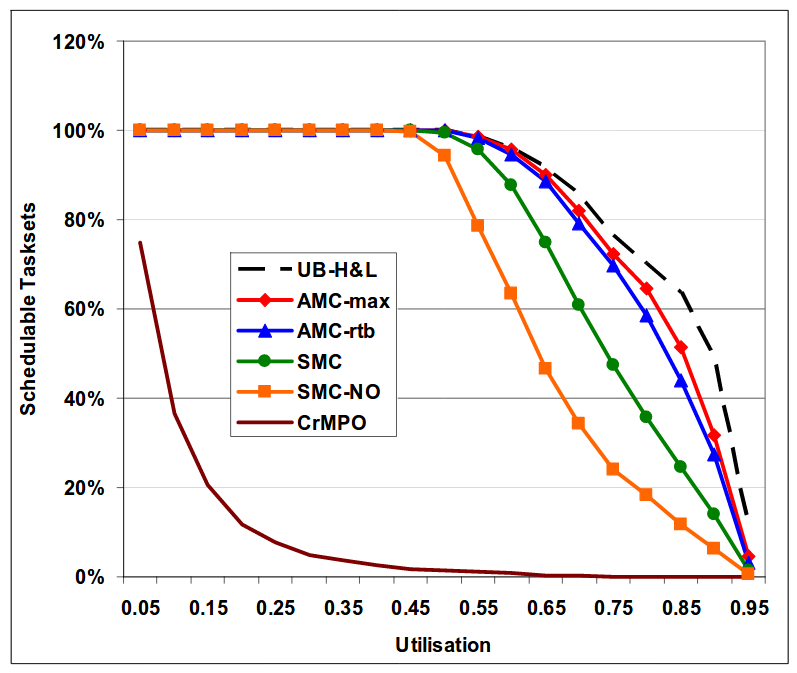
\includegraphics[width=\textwidth]{./img/literature_schedulers.png}
\caption{Percentage of schedulable tasks.~\cite{baruah2011}}\label{fig:schedulers}
\end{figure}

For a more complete review of work done on MCSs with a shared processor, see the paper by Burns~\cite{burns2016}.

%\subsection{Different criticality on different processors}


%\subsection{Sharing memory}
%http://pertsserver.cs.uiuc.edu/~mcaccamo/papers/euromicro12.pdf

\section{Standards}
%Different standards to regulate and ensure safety
Safety practices are becoming more regulated as industries adopt a standardized set of practices for designing and testing products. %TODO: expand, wording

\subsection{IEC 61508}
IEC 61508~\cite{IEC61508} is intended to be a basic functional safety standard for electrical and electronic systems applicable to all kinds of industry. It defines four different safety integrity levels, SIL~1 being the least dependable up to SIL~4 which is the most dependable level.

\subsection{ISO 26262}
ISO 26262~\cite{ISO26262} addresses the needs for an automotive-specific international standard that focuses on safety critical components. ISO 26262 is a derivative of IEC 61508.

\subsubsection{ASILs}
%ASIL QM (quality management) relates to the lowest (no) hazard, and ASIL
ISO 26262 describes five different Automotive Safety Integrity Levels (ASIL) relating to hazard and risk. Ranked from lowest (no) hazard to highest hazard, these levels are: QM, A, B, C and D. A function is assigned an ASIL depending on the severity if the function fails, the probability that the function fails and the controllability of the function, see table~\ref{table:ASIL}.

\begin{table}[H]
\centering
\begin{tabular}{|c|c|c|c|c|}
\hline
\multirow{2}{*}{\textbf{Severity}} &\multirow{2}{*}{\textbf{Probability}} &\multicolumn{3}{|c|}{\textbf{Controllability}} \\ \cline{3-5}
 & &C1 &C2 &C3 \\ \hline
\multirow{4}{*}{S1} & E1 & QM & QM & QM \\ \cline{2-5}
 & E2 & QM & QM & QM \\ \cline{2-5}
 & E3 & QM & QM & A \\ \cline{2-5}
 & E4 & QM & A & B \\ \hline
\multirow{4}{*}{S2} & E1 & QM & QM & QM \\ \cline{2-5}
 & E2 & QM & QM & A \\ \cline{2-5}
 & E3 & QM & A & B \\ \cline{2-5}
 & E4 & A & B & C \\ \hline
\multirow{4}{*}{S3} & E1 & QM & QM & A \\ \cline{2-5}
 & E2 & QM & A & B \\ \cline{2-5}
 & E3 & A & B & C \\ \cline{2-5}
 & E4 & B & C & D \\ \hline
\end{tabular}
\caption{ASIL as a function of severity, probability and controllability.}
\label{table:ASIL}
\end{table}

The various integrity levels can be translated into integers (ASIL $QM = 0$; $A = 1$; $B = 2$; $C = 3$ and $D = 4$). If a hazard requires several components to fail, the added ASIL of these components is used to determine if there is an violation, assuming the components faults are statistically independent of each other. For example, a safety level ASIL B can be met by two independent components which each individually only meet ASIL A (and thus effectively $A + A = B$).~\cite{azevedo2014} \\ %TODO: semi Wording

The different ASILs can relate to cost according to various cost heuristics, see table~\ref{table:cost_heuritics}. %TODO: Expand, wording

\begin{table}[H]
\centering
\begin{tabular}{|c|c|c|c|c|c|}
\hline
\textbf{Cost Heuristic} & \textbf{QM} & \textbf{A} & \textbf{B} & \textbf{C} & \textbf{D} \\ \hline
Linear & 0 & 10 & 20 & 30 & 40 \\ \hline
Logarithmic & 0 & 10 & 100 & 1000 & 10000 \\ \hline
Experimental-I~\cite{azevedo2014} & 0 & 10 & 20 & 40 & 50 \\ \hline
Experimental-II~\cite{azevedo2014} & 0 & 20 & 30 & 45 & 55 \\ \hline
\end{tabular}
\caption{ASIL cost heuristics.}
\label{table:cost_heuritics}
\end{table}


\subsubsection{Freedom from interference}
%TODO: Källa, utveckla, wording
In ISO 26262, Part 1, Definition 1.49, freedom from interference is defined as: Absence of cascading failures between two or more elements that could lead to the violation of a safety requirement. A cascading failure is defined as "failure of an element of an item causing another element or elements of the same item to fail" (ISO 26262, Part 1, Definition 1.13), and an element is defined as: "system or part of a system including components, hardware, software, hardware parts, and software units" (ISO 26262, Part 1, Definition 1.32)

\subsection{AUTOSAR}
%TODO: Wording
"AUTOSAR (AUTomotive Open System ARchitecture) is a international development partnership of automotive interested parties founded in 2003. It pursues the objective of creating and establishing an open and standardized software architecture for automotive electronic control units (ECUs) excluding infotainment. Goals include the scalability to different vehicle and platform variants, transferability of software, the consideration of availability and safety requirements, a collaboration between various partners, sustainable utilization of natural resources, maintainability throughout the whole "Product Life Cycle"."~\cite{website:autosar}\\

The AUTOSAR Architecture distinguishes on the highest abstraction level between three software layers: Application, Runtime Environment (RTE) and Basic Software (BSW) which run on a Microcontroller.~\cite{website:autosar} See figure \ref{fig:autosar}.
\begin{itemize}
\item The application software layer is mostly hardware independent.
\item The RTE represents the full interface for applications.
\item The BSW is divided in three major layers and Complex Drivers: Services, ECU Abstraction and Microcontroller Abstraction. Services are divided furthermore into functional groups representing the infrastructure for System, Memory and Communication Services.
\end{itemize}

\begin{figure}[H]
\centering
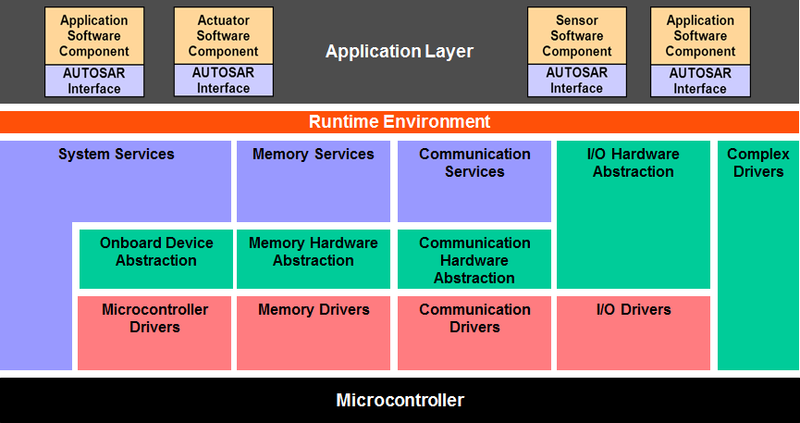
\includegraphics[width=\textwidth]{./img/literature_autosar.png}
\caption{AUTOSAR.~\cite{website:autosar}}\label{fig:autosar}
\end{figure}

\section{Mixed criticality platform solutions}
%Literature study about platfrom solutions for MCS

\subsection{Hypervisors}
A virtual machine monitor, or hypervisor, can be seen as an interface between the operative systems and the hardware of a system. In order to facilitate for multiple operative systems of different criticality an appropriate hypervisor bla bla. A system will only be as secure as its hypervisor. Some hypervisors can accommodate multiple instances of operative systems, and some only facilitate for two. A description of a few available open-source hypervisors will follow.

\subsubsection{SafeG}
TOPPERS group of Nagoya University in Japan has developed an open-source dual-OS architecture designed to concurrently host a real-time operating system (RTOS) and a general purpose operating system (GPOS) on TrustZone enabled ARM SoC devices [34]. SafeG takes advantage of ARM’s TrustZone security extensions to efficiently partition the system into Trusted and Non-Trusted states, which provides full system access to trusted software, and limits the capabilities of software running in Non-Trusted state. SafeG includes the following features:

Enables the concurrent execution of RTOS and GPOS on either single-core or multi-core ARM-based platforms.

Devices and memory regions that are configured as Secure are protected against illegal GPOS accesses.

Normal world devices can be accessed from both GPOS (Non-Trusted) and RTOS (Trusted) software.

Real-time requirements are guaranteed in RTOS (Trusted) via the utilization of FIQ and IRQ interrupts, where FIQ interrupts are issued for RTOS and IRQ interrupts are issued for GPOS. While in the Trusted state, IRQ interrupts are disabled so that GPOS can not disturb the execution of the RTOS. Therefore, GPOS only executes when the RTOS issues the Secure Monitor Call (SMC) instruction, which causes the SafeG monitor to switch from the Trusted world (RTOS) to the Non-Trusted world (GPOS). Furthermore, FIQ interrupts are active during the execution of GPOS, which enables RTOS to retake control of the system. For example, a cyclic execution of RTOS/GPOS can be controlled by an FIQ interrupt of a system timer.

GPOS does not require any major changes, and can execute with minimal overhead.

Includes an efficient guest-to-guest communication mechanism (i.e.referred to as SafeG COM)

Figure 5.1 depicts the SafeG architecture. It shows a simplified view of a TrustZone enabled ARM processor together with partitioned memory and device IO. The memory and device IO are configured as either Trusted (Secure) or Non-Trusted (Non-Secure), and their access is controlled by the NS bit of the bus (see subsection 3.2.9). The SafeG Monitor is the gateway between the GPOS and the RTOS. During the switch operation, it is responsible for saving the state of one world and loading the state of the other. The RTOS tasks are statically mapped to each processor during compilation. On the other hand, the GPOS uses all available virtual CPUs in SMP (Symmetric Multi-Processor) mode. Furthermore, the GPOS does not have access to Secure memory regions and Secure device IO. However, the RTOS can access all system resources. Therefore, by designating a resource as Non-Secure and making the RTOS aware of its existance, both the GPOS and RTOS can gain access, which is essential for communication between the two regions.

\subsubsection{SICS Thin hypervisor}
SICS Thin Hypervisor (STH) is a light-weight hypervisor designed for ARM-
based devices [35]. STH runs directly on top of the hardware (bare metal),
and achieves system virtualization through paravirtualization. As a result,
guest systems require some modifications to the OS kernel, including the
addition of a hypercall * inteface. STH strengthens the security of embedded
systems through the isolation capabilities of virtual machines, and allows
for the existence of heterogeneous operating systems on the same platform.
Current STH version supports ARMv5 (926EJ-S) and ARMv7 Cortex-A8
only. However, STH is a highly flexible and portable hypervisor that uses a
hardware abstraction layer with minimal size.

\subsubsection{Sierra visor}
Sierraware offers a bare metal universal hypervisor (SierraVisor) that is
available as open-source under the GNU GPL v2 license or with a commercial
license [33]. It supports paravirtualization, TrustZone virtualization, and
hardware assisted virtualization. SierraVisor is compatible with Cortex-
A9/A15 and ARM11 based SoCs, but only Cortex-A15 supports the
hardware assisted virtualization option * . The TrustZone virtualization
approach allows for the integration of guest operating systems without any
kernel modifications. Each guest kernel and applications run in their usual
privilege mode, supervisor and user mode respectively. Furthermore, each
guest executes in an isolated container with low overhead.

\subsubsection{Xen hypervisor}
The Xen hypervisor is widely used in enterprise and is now making its way
to embedded systems. It was developed in Cambridge University, and is
available as open-source software under the the general public license (GNU).
The Xen hypervisor is implemented as the guest console architecture, as
discussed in subsection 4.2.4. The hypervisor layer is a thin software layer
that resides above the hardware layer. It is the first program that runs
after the bootloader, and is responsible for managing the CPU, Memory, and
interrupts.
By default, the Xen hypervisor uses Credit as the CPU scheduler, which
allows the user to allocate a percentage of the CPU time for each VM, or allow
the hypervisor to automatically balance the workload across active CPUs in
the system. Alternatively, the user can specify Simple Earliest Deadline First
(SEDF) algorithm for the scheduler. However, the load-balancing feature will
be unavailable [28].
The hypervisor is responsible for launches Dom0, which is a special virtual
machine that has privileged access rights to the physical I/O resources. It
handles I/O accesses and interacts with the other virtual machines. All other
VM instances operate in Domain U (DomU), which runs in unprivileged mode. The guest virtual machines can be either paravirtualized (PV) or
fully virtualized {a.k.a. Hardware-assisted Virtual Machine (HVM)}. The
PV guest are modified operating systems such as: Linux, Solaris, FreeBSD,
or other UNIX operating systems. In order to facilitate I/O sharing, Xen
uses split-driver architecture. This approach manges I/O accesses of DomU
PV guests. The split-driver technique divides the driver into a front-end,
located in the DomU PV guest, and a back-end, located in the Dom0 guest.
DomU PV guests are aware that they do not have direct access to the
hardware and that they are running alongside other virtual machines on the
same hardware. However, DomU HVM guests are unaware of the presence
of other VMs, and of the fact that they are sharing hardware resources.
Instead of split-drivers, in the HVM architecture, a special daemon is started
in Dom0 guest for each DomU HVM guest. The Xen hypervisor is available
for both Intel and ARM devices. However, it is not recommended to use Xen
with devices that do not contain IOMMU units because the hypervisor can
be easily subverted by DMA capable devices [29].

\subsubsection{Xen zynq}
The open-source Xen hypervisor has recently been ported to the new
Xilinx Zynq Ultrascale+Multi-Processor System-on-Chip (MPSoC) device
[30]. Xen Zynq Distribution is released under the GNU General Purpose
License 2 (GPL2). The processing platform features a quad-core ARM
Cortex-A53, a dual-core ARM Cortex-R5, a Mali-400MP2 GPU, and FPGA
fabric that supports run-time reconfiguration. This device is the successor of
Xilinx Zynq SoC, which features a dual-core Cortex-A9 processor and FPGA
fabric.

\subsubsection{SEL4 microkernel}
The sel4 microkernel is based on the L4 microkernel, which is one of the
smallest kernels available today. Sel4 is the first formally verified microkernel,
which implies that its specification is verified mathematically. Sel follows
the ”minimality principle”, which dictates that the kernel shall only contain
functionalities that can not be implemented at the user-level [31]. As a result,
the microkernel is small, efficient, and robust. All device drivers are excluded
from the microkernel level and execute in unprivileged mode, except for a
timer driver and an interrupt controller driver.
The microkernel supports a small number of services that enable applicationsto create and manage threads, virtual memory spaces, and interprocess
communication (IPC). Furthermore, sel4 follows a ”capability-based access
control model” in order to manage the access rights to all kernel services.
Capabilities are unforgeable tokens that contain metadata about a specific
kernel object, including its access rights. The use of capabilities as a control
mechanism allows the system to maintain strong isolation between software
components [32].
The sel4 microkernel implements a fixed-priority round-robin scheduler
policy, mainly because its current ”time” abstraction method is under-
developed and does not yield satisfactory results. As proposed in [31],
reservations can be added to sel4 in order to provide a suitable temporal
isolation solution for real-time systems.
Sel4 provides IOMMU support for Intel-based architectures (IA-32),
which allows the safe integration of DMA enabled devices. Furthermore,
Sel4 can support multicore systems via multikernel bootstrapping. However,
this feature is only available for x86 machines; only uniprocessor is supported
for ARM-based devices.


\section{Platooning}
%TODO: wording
Platooning, road trains or convoy driving is the concept of a chain of vehicles traveling at a given (short) intermediate distance in order to utilize the reduced air friction behind the vehicle in front. The primary objective for each vehicle with respect to safety is to maintain its distance to the preceding vehicle in the platoon.

\subsection{Benefits of platooning}
%TODO: Expand, wording, source
Potential benefits of vehicle platooning includes lower fuel consumption, less road space required and more efficient traffic flow.\\ 

Using simulations of platooning, Alam, Gattami, and Johansson \cite{johansson2010} showed in 2010 that there is a \mbox{4.7--7.7\%} fuel reduction potential in heavy duty vehicle platooning at a set speed of 70 km/h with two identical trucks.\\

In 2014, Lammert et. al.~\cite{lammert2014} showed in tests that platooning can result in reduced fuel consumption of up to 5.3\% for the lead vehicle and up to 9.7\% for following vehicles.\\

Tests by truck manufacturer Scania have shown that platooning can reduce fuel consumption by up to 12\%~\cite{scania2015}.

\subsection{Safety requirements for platooning}
%more sources
With shorter distance between vehicles, the margin of error also decreases. This puts high requirements on the system controlling the speed of the vehicles in the platoon.\\

In the article by Alam et al.~\cite{johansson2013}, safe sets for heavy duty vehicle platooning are computed to calculate minimum distance between the  vehicles in a platoon without endangering safety. System uncertainties or varying vehicle parameters, such as mass, air resistance and road gradient, could cause a difference in braking capabilities between the vehicles, thereby changing the shape of the safe sets. If the follower vehicle has a higher braking capacity, it will be able to lie closer without endangering a collision. The minimum safe relative distance is therefore shorter compared to the case of two identical vehicles. However, if the lead vehicle has a greater braking capability the relative distance must be increased significantly. Delays for the platoon control system commonly occur due to detection, transmission, computation, and producing the control command. A delay in the system implies that the lead vehicle will be able to act, change the relative velocity and distance, before the follower vehicle is able to react. A delay can be translated into a shift of the reachable set. However, no change occurs in the follower vehicle's velocity, since it does not react. Depending on the radar and the collision detection algorithm, a worst-case delay is approximately 500~ms for the considered vehicles. Hence, the lead vehicle will be able to reduce the relative velocity by 3.25~m/s and the relative distance by 0.8~m if it is driving 25~m/s at normal mode. Thus if the follower vehicle maintains a distance of at least 2~m, a collision can always be avoided for two identical vehicles~\cite{johansson2013}.

\section{Lane detection and lateral control}
%
\chapter{Alten MCS}
\label{sec:lit_emc2mcs}
%Describe current system more in depth.
%This chapter will describe the EMC\textsuperscript{2} development platform, for more information see the report by Zaki~\cite{zaki2016}.
This chapter will describe the Alten MCS, its different components and how it is built.

\section{Overview}
The Alten MCS (Alten Mixed Criticality System) is a Mixed Criticality System consisting of both hardware and software components. The general idea is that it should be capable of running two operating systems of different criticality on the same hardware, separated via a hypervisor, where errors from the non-critical OS should not be able to propagate into the safety-critical OS. The Alten MCS has currently been built on two different development boards, the EMC\textsuperscript{2} Development Platform (EMC\textsuperscript{2}DP) and the Zynq Evaluation and Development board (Zedboard). Both boards are equipped with a Zynq-7000 System on Chip (SoC). The development boards can be seen in Figure~\ref{fig:development_boards}.

\begin{figure}[H]
\centering
\begin{subfigure}[b]{0.3\textwidth}
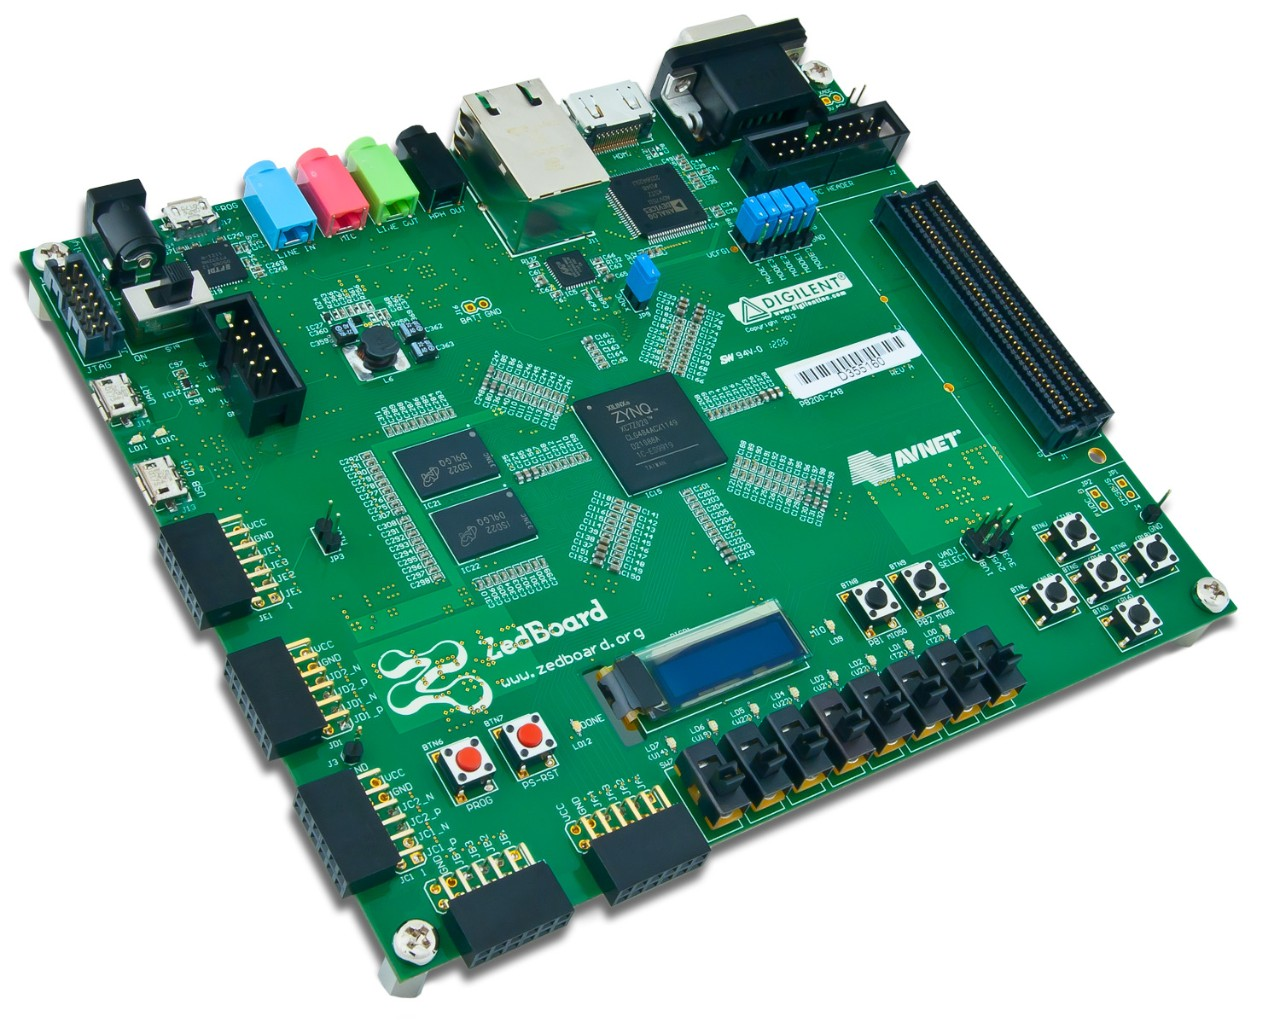
\includegraphics[width=\textwidth]{./img/zedboard.jpg}
\caption{Zedboard}
\end{subfigure}
\begin{subfigure}[b]{0.3\textwidth}
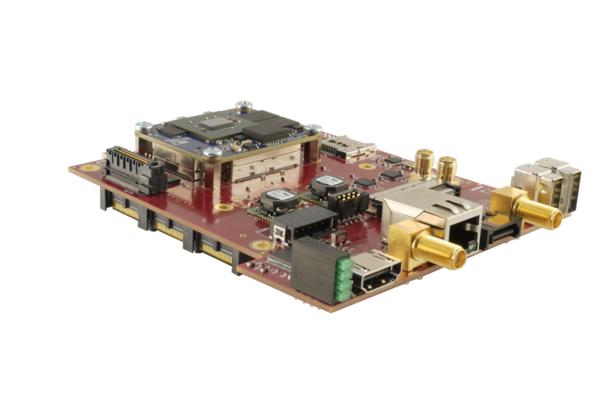
\includegraphics[width=\textwidth]{./img/emc2dp.jpg}
\caption{EMC\textsuperscript{2}DP}
\end{subfigure}
\caption{}
\label{fig:development_boards}
\end{figure}

\section{Hardware}
The Zynq-7000 SoC has a Processing System (PS) consisting of a hardwired application processing unit, memory controller, and peripheral devices. The main processing unit is a dual-core Cortex-A9 ARM processor. Connected to the PS region is a Programmable Logic (PL) region. The PL is based on Xilinx’s 7-series FPGA technology.\\

Both the PS and PL regions have support for ARM TrustZone~\cite{website:ARM}.

\section{Operative systems}
The Alten MCS uses two Operative Systems (OS) to create temporal and spatial separation between safety-critical and non-critical applications using TrustZone. In its current setup the Real-Time Operative System (RTOS) FMP by TOPPERS~\cite{website:fmp} is used for safety-critical applications. This RTOS follows the uITRON4.0 specification~\cite{uitron}, which is a widely used RTOS specification for Japanese embedded systems. For non-critical applications, the General Purpose Operative System (GPOS) Linux kernel 4.4 is used. Instead of Linux another instance of FMP could be used for non-critical applications.\\

Tasks in FMP are statically allocated to a processor core, defined in a .cfg file. Linux divides its workload across all available processor cores in SMP (Symmetric Multi-Processor) mode.

\section{Hypervisor}
%TODO: timings for switching
%The hypervisor SafeG is used to alternate between the safety-critical (S\_OS) and non-critical (NS\_OS) OS. It switches processor state via a hardware switch. See figure~\ref{fig:modeswitch}. The switching takes ~2 $\mu s$.

A hypervisor (also known as a Virtual Machine Monitor (VMM)) is used to alternate between the safety-critical (S\_OS) and non-critical (NS\_OS) OS. The hypervisor used is SafeG \cite{website:safeg}, also developed by TOPPERS. It switches processor state via a hardware switch. See figure~\ref{fig:modeswitch}. The switching takes roughly 2~$\mu s$~\cite{safegswitch}.

\begin{figure}[H]
\centering
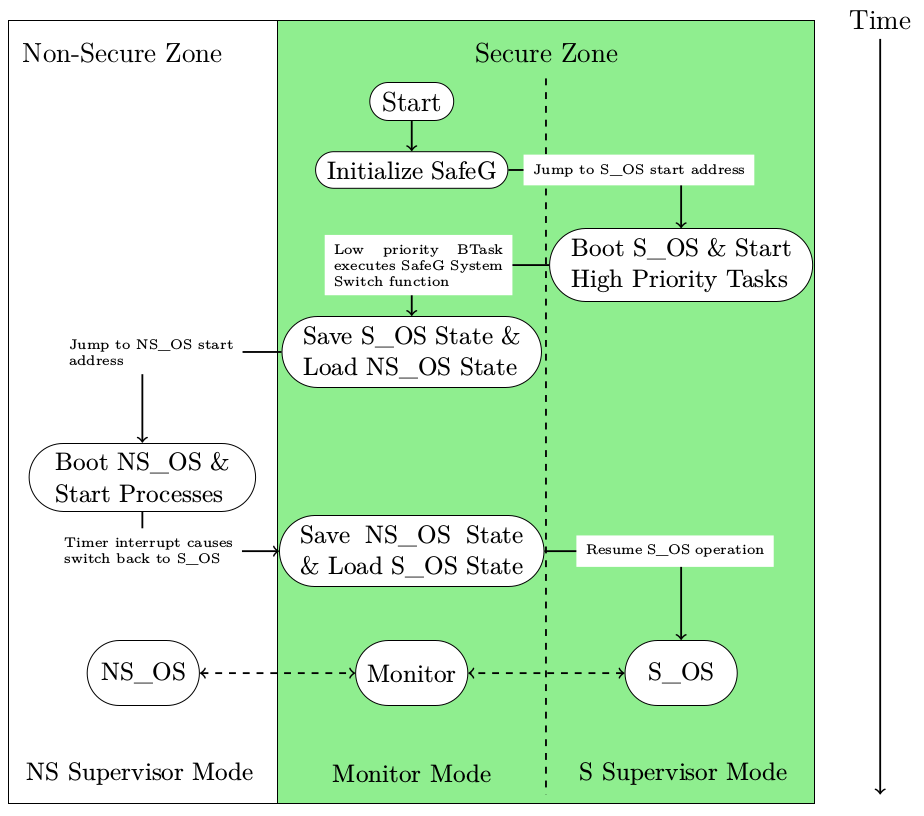
\includegraphics[width=\textwidth]{./img/literature_modeswitch.png}
%Flowchart of how the physical CPU switches between the virtual CPUs
\caption{Flowchart of the boot sequence of the CPU. \cite{zaki2016}}\label{fig:modeswitch}
\end{figure}

%TODO: gör okefft
%As far as the hypervisor is concerned, the GPOS is another task with lowest priority. \\
When executing the tasks via the hypervisor, all S\_OS tasks are executed according to the scheduling. At the lowest priority is the task that switches processor state. As soon as an S\_OS task needs to execute, a FIQ is issued to interrupt the processor and switch mode back to the S\_OS. \\

The time it takes the hypervisor to switch processor state bounds the theoretical maximum frequency a cyclic task can have while the processor still manages to maintain its switching capabilities. The maximum frequency, $f_{max}$, can be calculated as

\begin{equation} \label{eq:max_frequency}
f_{max} = \lim_{e_s, e_{ns} \to 0} \frac{1}{e_s+e_{ns}+2e_{switch}}
\end{equation}

where $e_s$ is the execution time of the tasks on the S\_OS, $e_{ns}$ is the execution time of the tasks on the NS\_OS and $e_{switch}$ is the time required for the mode-switch.\\

A more practical limitation is that the periodicity of a cyclic task in FMP is defined by an integer in milliseconds, meaning that the highest frequency for a periodic task is $1\textrm{ kHz}$.\\

A basic overview of the hardware and the software of the system can be seen in Figure~\ref{fig:system_overview}.

\begin{figure}[H]
\centering
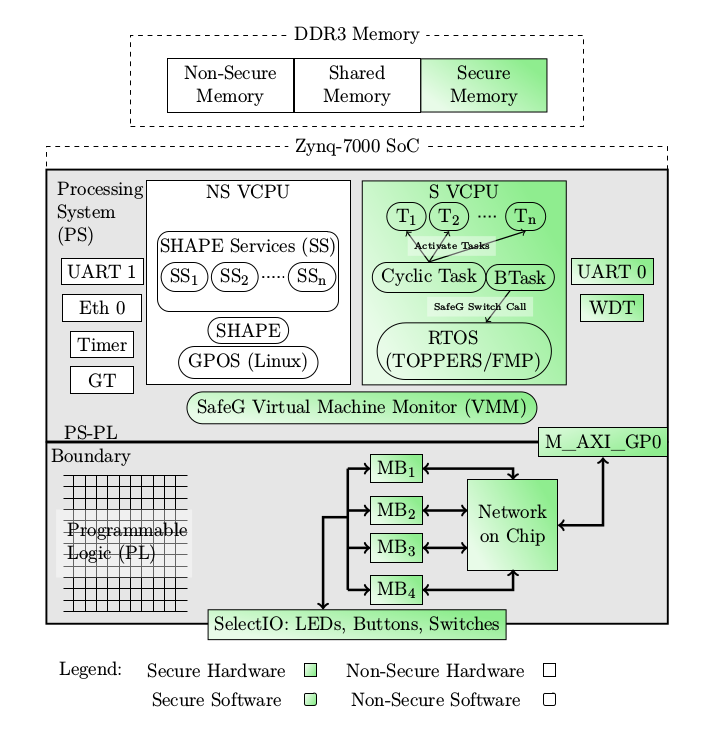
\includegraphics[width=\textwidth]{./img/system_overview.png}
\caption{Overview of the Alten MCS.\cite{zaki2016}}\label{fig:system_overview}
\end{figure}

\section{Build procedure}
The MCS is built from many different components. Hardware design, applications, virtualization layer, operative systems, boot loaders etc. This section will describe the build procedure.\\ %TODO: Expand
%The virtualization layer (SafeG) and the Secure OS (RTOS) remain the same, the software that runs in the normal region can be either RTOS, GPOS, or a bare metal application. Furthermore, other configurations, such as RTOS or GPOS only mode, do not include the VMM.

Xilinx's software Vivado HLS~\cite{website:vivado} is used to design the FPGA of the Zynq-7000. In Vivado the different IPs, their interconnect and the Processing System is configured. This results in a bitstream file that is used in Xilinx SDK to generate a Board Support Package (BSP) and the First Stage Boot Loader (FSBL). The BSP contains libraries for functions and variables necessary for the IPs on the FPGA, and the FSBL configures the FPGA correctly. The FSBL is included in a boot file (BOOT.bin) generated in Xilinx SDK. The boot file is loaded to an SD card that is inserted into the development board. When powered up, the Zynq-7000 boots from the SD card and configures the FPGA according to the FSBL and loads the Second Stage Boot Loader (SSBL), u-boot, which also is contained in the boot.bin file. U-boot is a program that can load executables and other system files from a remote server into the DDR3 memory. This is used to load relevant files for the OS into the Zynq, which brings us to the software part of the build procedure. The software is divided into three parts: RTOS, GPOS and monitor. The SafeG monitor is built and compiled using GCC (Gnu Compiler Collection), resulting in monitor.bin. The RTOS FMP is built and compiled from a .cfg file where tasks and handlers are created, a .c file where tasks and handlers are defined and a .h file containing declarations. This results in fmp.bin. For the non-secure side either Linux or another instance of FMP could be used. The process for FMP is the same as with the secure side. For Linux on the non-secure side, the Linux kernel needs to be modified to support SafeG. This results in the files zImage, devicetree.dtb. All of these files are created and stored on a server and are then loaded into the Zynq-7000 using u-boot.\\

%Xilinx's software Vivado~\cite{website:vivado} is used to synthesize the hardware design (vhdl or verilog code) into a bitstream file (.bit) in order to configure the PL region of the Zynq. Vivado also produces a set of files that represent the designed hardware platform, which are used for software development. Xilinx SDK tool is used to create the Board Support Package (BSP) and the First Stage Boot Loader (FSBL) that correspond to the designed system. In general, after the FSBL initialization process completes, and depending on boot sequence, the CPU can do any of the following actions: configure the FPGA, initiate the Second Stage Boot Loader SSBL, or jumps to the first address of the main program. The SDK tool is also used to generate a boot file (BOOT.bin), which must at least contain the FSBL (fsbl.elf). In the implemented system, the BOOT.bin file also includes the bitstream file (system.bit) and the SSBL (uboot.elf * ). Once the system is initialized and the PL is configured, the system starts executing the u-boot instructions present in the BOOT.bin. U-boot is a full system on its own, and has many useful features. In particular, u-boot can be used to load executables and other system files from a remote server into the DDR3 memory using protocols such as Trivial File Transfer Protocol (TFTP), see Figure~\ref{fig:system_build}.\\

Figure \ref{fig:system_build} provides a summary of the different dependencies for the system and the required flow for building the system.

%TODO: NY BILD

\begin{figure}[H]
\centering
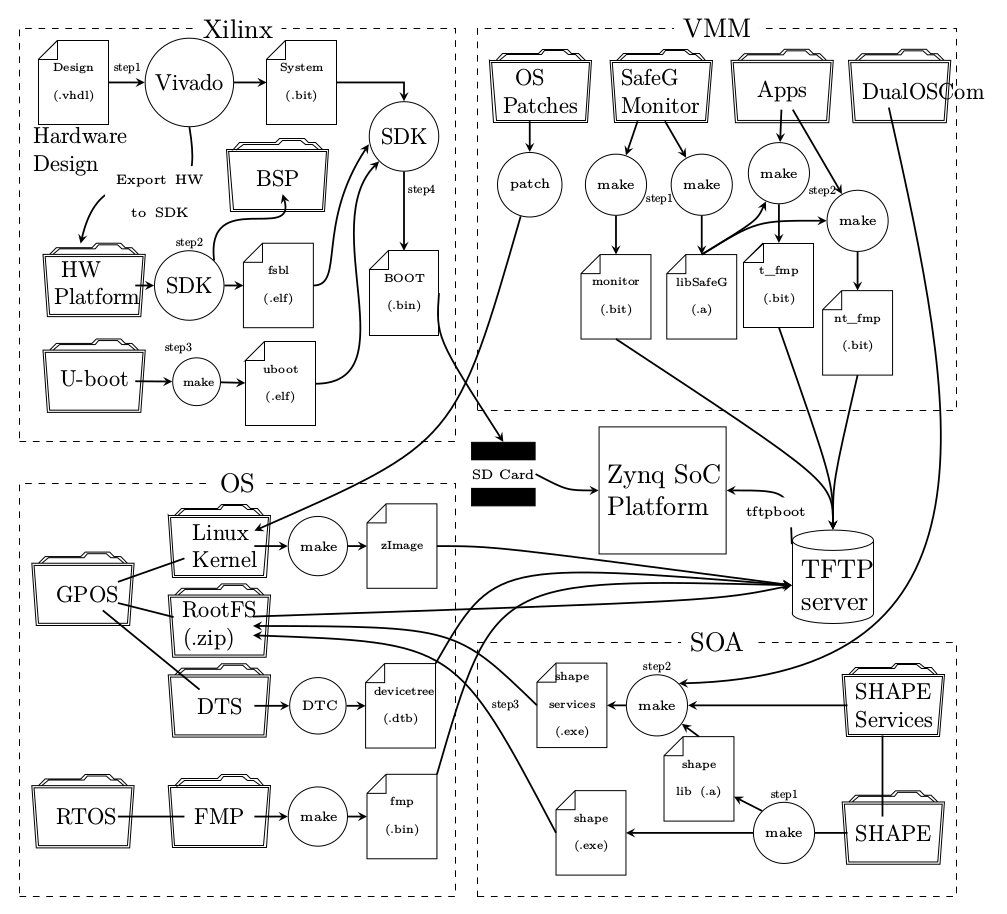
\includegraphics[width=\textwidth]{./img/literature_build.png}
\caption{System build procedure.\cite{zaki2016}}\label{fig:system_build}
\end{figure}

%For more information about the build and the system, see the report by Zaki~\cite{zaki2016}.

This build procedure setup provides for easy modifications to a small part of the system without having to rebuild other parts, and the board to which the code should be loaded into only needs to be connected to a network socket and a laptop.
%TODO: rephrase
\chapter{System design}
\label{sec:system_design}
%This chapter will derive the design of the system.
For the system to accomplish the goals stated in \ref{sec:problem}, several hardware and software functions need to be designed and implemented.\\

%For the mixed criticality implementation, the hypervisor SafeG~\ref{sec:safeg}~\cite{website:safeg} will be used to alternate between the safety-critical RTOS FMP and the GPOS, as described in section~\ref{sec:lit_emc2mcs}. Several safety-critical functions will run on FMP.

\section{Operative system functions}
This section will describe the functions to be implemented in the RTOS.

\subsection{Longitudinal control}
A controller will be implemented to control the speed of the vehicle and its distance to the vehicle in front of it. The controller will have three different modes, Cruise Control (CC), Adaptive Cruise Control (ACC), and Cooperative Adaptive Cruise Control (CACC). The CACC controller will use speed, distance to preceding vehicle and information communicated from the preceding vehicle as input to calculate a control signal. For an illustration of the controller architecture, see figure~\ref{fig:cacc}.\\

\begin{figure}[H]
\centering
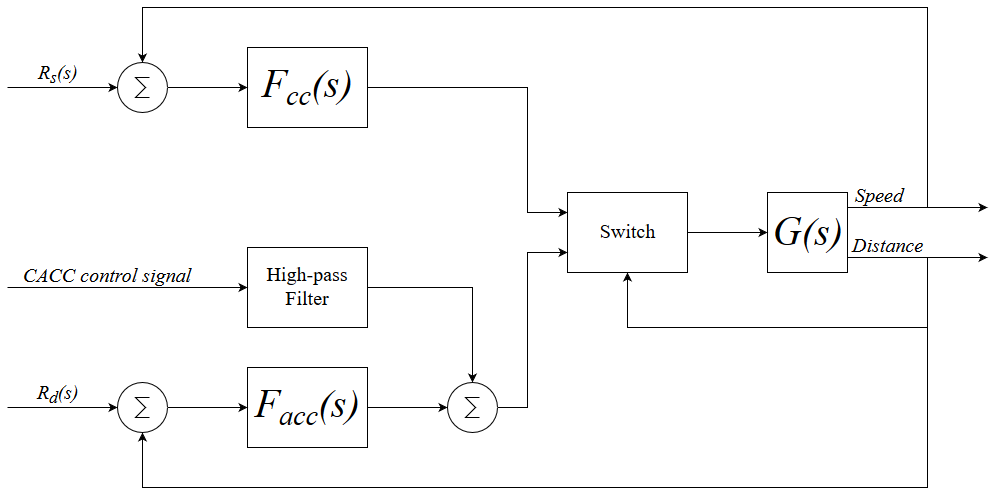
\includegraphics[width=\textwidth]{./img/design_cacc.png}
\caption{The architecture of the designed controller where $F_{cc}$ is a PID controller controlling the speed, $F_{acc}$ is a PID controller controlling the distance and G is the dynamics of the car.} \label{fig:cacc}
\end{figure}

For more information, see the report by Roshanghias~\cite{roshanghias2017}.

\subsection{Lateral control}
A lane-detecting algorithm will be implemented on a Raspberry Pi that will send data to the Alten MCS. The choice of Raspberry Pi was made because of the amount of open source video processing code available for the platform. For more info, see the report by Ferhatovic~\cite{ferhatovic2017}.\\

Lateral control will be implemented on the RTOS on the Alten MCS. The function receives the deviation from the center line as calculated by the lane detection algorithm from the Raspberry Pi, and calculates a control signal from this.

\subsection{Data aggregation}
This function will read wheel sensor data and calculate if the road conditions are unsafe for platooning. See the report by Hellman~\cite{hellman2017}.\\

The function will also serve as a filter for distance measurements and speed measurements for other tasks to use.

\subsection{Communication}
To maintain secure communication between the two vehicles in the platoon a communication protocol will be developed. For more information, see the report by Lerander~\cite{lerander2017}.% WiFi will be used to communicate wirelessly, and  WiFi messages will be parsed in a MicroBlaze processor in the FPGA and sent to the OS. 

%A WiFi module receives data and sends it via UART to a MicroBlaze processor on the FPGA where data is parsed and sent up to the OS via a mailbox. In the OS the mailbox is emptied and data is sent to where it is needed. The communication task then sends the data it should sent to the MicroBlaze where the data is packaged properly and sent as an UDP packet via the WiFi module. 

\section{Hardware implemented functions}
This section will describe the functions to be implemented on the FPGA, also known as IPs.

\subsection{Speed reading}
To read the speed of the vehicle, encoders need to be connected to the wheels. The four encoders will send pulses very quickly and a hardware decoder is needed to process them and send the speed of each wheel to the OS.

\subsection{Distance reading}
To read the distance to the preceding vehicle, a LIDAR (LIght Detection And Ranging) will be used. The LIDAR communicates the distance it is reading via a PWM signal. A hardware function is needed to read the PWM pulse and convert it to a distance.

\subsection{Communication}
WiFi communication is used between the two vehicles in the platoon. To read packages, a WiFi module is used that communicates via UART with the Alten MCS. A MicroBlaze in the FPGA processes the packages and sends the parsed data to the OS via a mailbox. For more information, see the report by Lerander~\cite{lerander2017}.

\subsection{Actuation}
To actuate control signals and thereby control the speed of the motor and the position of the steering servo, Pulse Width Modulation (PWM) is used. Two hardware implemented PWM functions will be needed for this.

\subsection{Raspberry Pi communication}
To receive information from the Raspberry Pi, some form of communication interface needs to be used. One simple solution for this is UART (Universal Asynchronous Receiver Transmitter) serial communication. 

\section{Overview design}
An overview of the different functions to be implemented on the Zynq-7000 can be seen in figure~\ref{fig:overview}.

\begin{figure}[H]
\centering
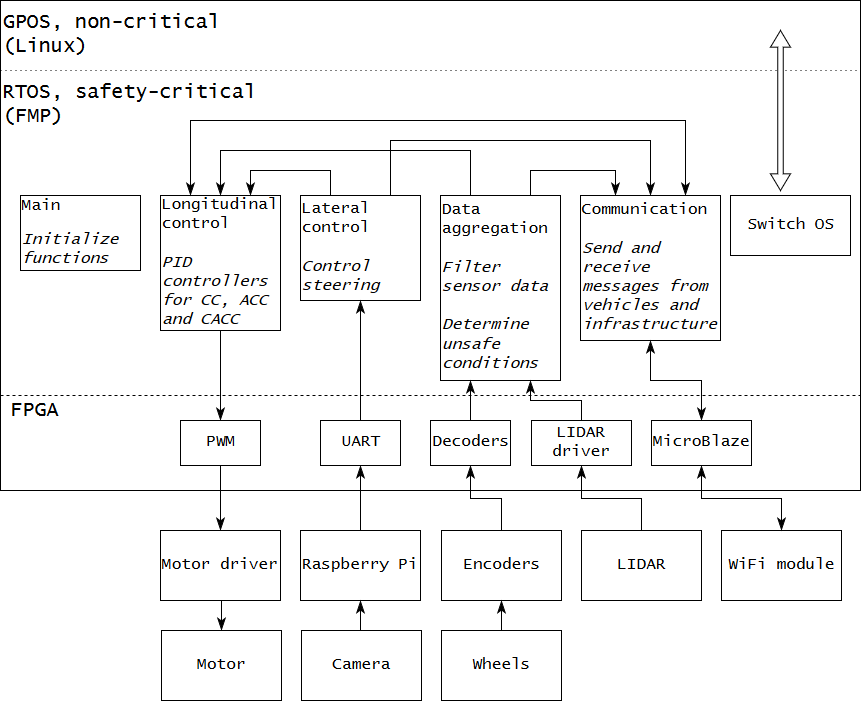
\includegraphics[width=\textwidth]{./img/design_overview.png}
\caption{Overview of the different functions to be implemented. The arrows indicate information flow between the different functions.}\label{fig:overview}
\end{figure}

A sequence diagram of the various dependencies and flow of each function can be seen in figure~\ref{fig:sequence}.

\begin{figure}[H]
\centering
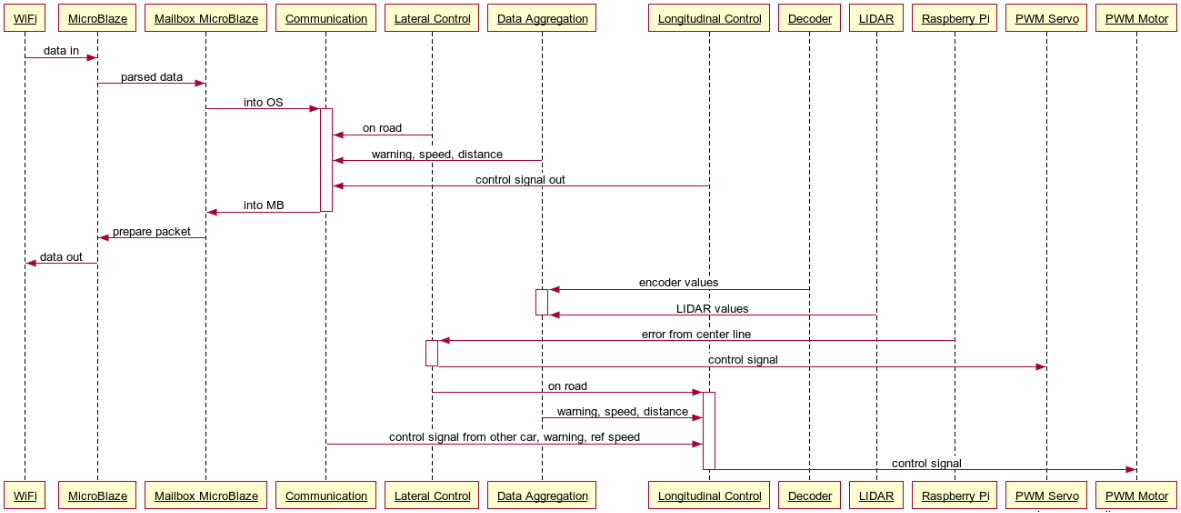
\includegraphics[width=\textwidth]{./img/design_sequence3.png}
\caption{Sequence diagram of the various hardware and software functions, their dependencies and flow of information.}\label{fig:sequence}
\end{figure}

\chapter{Implementation}
This chapter will describe the implementation of the entire system in the demonstrator.

\section{Platform}
To demonstrate the system, the RC car UTOR 8E from BSD racing was chosen. It is a 1/8 scale RC car with a steering servo, brushless DC motor, and most importantly, it was readily available from a local store.\\

For the demonstrator, it was decided to use the Zedboard on both vehicles for a number of reasons:
\begin{itemize}
\item The power supply connector for the EMC\textsuperscript{2}DP would have to be remade to be used in the vehicle.
\item Connections on the vehicles fitting the measurements of the Zedboard were made.
\item Same BSP for both vehicles.
%\item The Zedboard was all around easier to work with
\end{itemize}

The car with all of its components can be seen in figure~\ref{fig:utor_overview}.

\begin{figure}[H]
\centering
\includegraphics[width=\textwidth]{./img/implementation_utor.png}
\caption{One of the two vehicles on the test track. Visible in the picture is the LIDAR in the front, the Raspberry Pi and its camera. The Zedboard can be seen under the covering plastic glass.}
\label{fig:utor_overview}
\end{figure}

\subsection{Driver}
The driver for the motor and steering servo is controlled by a PWM signal with a frequency of 50~Hz. The speed is controlled by the pulse length of the PWM signal. This was tested with the hand-controller to see what PWM signals were received at the end points. Maximum and minimum high time measured was 2~ms and 1~ms, which at 50 Hz corresponds to a duty cycle of 10 and 5 \%. Depending on how high frequencies the driver could handle, the frequency could be increased without changing the high time, potentially up until a period of 0.02 seconds would make the maximum signal correspond to a duty cycle of 100\%.\\

This was tested, and gave somewhat expected results. The driver had some disturbances and gave maximum or minimum output sporadically when it shouldn't, with more disturbances at higher frequencies. It was decided that a frequency of 50 Hz would have to do.

\section{Electrical wiring}
The electrical power for all components on the car is sourced from the battery pack: two 7.4V batteries in parallel. Three voltage regulators are connected to the batteries to give power to other components. 

\begin{itemize}

\item 7.4V to 5V for LIDAR, Encoders and Raspberry Pi.

\item 7.4V to 5V for WiFi module.

\item 7.4V for DC input voltage for Zedboard. (Here the voltage regulator only acts as a filter.)

\end{itemize}

The WiFi module was put separately from the other 5V output since it draws too much current to be combined with the other components for one voltage regulator to handle. 

\section{RTOS tasks}
This section will describe the task implemented on the RTOS.

\subsection{Data aggregation}
The task \texttt{data\_aggregation()} is the task with the highest frequency in the system. It executes with a period of 1 ms, which the shortest period allowed in FMP. It reads the speed from each wheel as measured by the decoder, and analyses if the road conditions are unsafe for platooning. It also filters speed and distance measurements through a low-pass filter to produce reliable data for the other tasks to use.

\subsection{Communication}
The task \texttt{communication()} reads V2V and I2V messages stored in a buffer on the FPGA. The messages are unpacked and forwarded to their intended destination task. Information from the other tasks are sent the to the FPGA. The task \texttt{communication()} is bounded by the period of the larger communication loop and the period of \texttt{lateral\_control()} and \texttt{longitudinal\_control()}. It can only send messages with a period of 800 ms. Since the received messages are stored in a buffer on the FPGA, the task only needs to execute before every execution of \texttt{lateral\_control()} and \texttt{longitudinal\_control()}. This puts its period at 20~ms.

\subsection{Lateral control}
The task \texttt{lateral\_control()} receives angle and positional error of the vehicle in relation to the detected lane and computed a control signal via a PID controller. The task also sends lane detection status to \texttt{longitudinal\_control()}. Due to the limitations by the PWM described earlier the control frequency was capped at 50 Hz, meaning a period of 20 ms.

\subsection{Longitudinal control}
Just like \texttt{lateral\_control()}, the period of \texttt{longitudinal\_control()} is 20 ms. The task consists of two PID controllers, one for CC and one for ACC (as described in chapter~\ref{sec:system_design}). The controller adds the control signal from the preceding vehicle to its own control signal if secure communication is established and the vehicles are in platoon/CACC mode. It also sends its control signal to the \texttt{communication()} task. If the lane detection status received from \texttt{lateral\_control()} indicates that no lane is detected, \texttt{longitudinal\_control()} stops the vehicle.

\section{GPOS}
Linux was run on the non-secure side. From the beginning there were ideas of hosting a video feed from the camera on the vehicle, but there was not nearly enough time to implement this. Instead, the Linux was running idle and was only used to navigate the file system to demonstrate that it was in fact up and running. 

\section{Processor scheduling}
The above tasks with their required period and WCET as can be seen in chapter~\ref{sec:results} resulted in the processor scheduling seen in figure~\ref{fig:rtsched}.

\begin{figure}[H]
\centering
\begin{RTGrid}[nonumbers=1]{6}{25}

%Data aggregation
\TaskNArrival{1}{0}{7}{4}
\TaskNExecDelta{1}{0}{1}{7}{4}

%Communication
\TaskArrival{2}{0}
\TaskRespTime{2}{0}{1}
\TaskExecution{2}{1}{2}

%Lateral control
\TaskArrival{3}{0}
\TaskRespTime{3}{0}{2}
\TaskExecution{3}{2}{3}

%Longitudinal control
\TaskArrival{4}{0}
\TaskRespTime{4}{0}{3}
\TaskExecution{4}{3}{4}

\TaskExecution{5}{4}{5}

%OS switch
\TaskNExecDelta{5}{6}{1}{7}{3}
\TaskNExecDelta{5}{8}{1}{7}{3}

%GPOS
\TaskRespTime{6}{0}{25}
\TaskExecution{6}{5}{6}
\TaskNExecDelta{6}{9}{4}{7}{2}
\TaskExecution{6}{23}{25}

\end{RTGrid}
\caption{Processor scheduling, not to scale.}\label{fig:rtsched}
\begin{tabular}{r@{: }l r@{: }l r@{: }l}
$\tau_1$ & Data aggregation & $\tau_2$ & Communication & $\tau_3$ & Lateral control\\
$\tau_4$ & Longitudinal control & $\tau_5$ & OS switch & $\tau_6$ & GPOS
\end{tabular}
\end{figure}

\section{Hardware functions}
This section will describe the implementation of the hardware functions, or FPGA IPs. For the entire Vivado block design showing the FPGA IPs and their interconnect, see Appendix~A.

\subsection{Pulse Width Modulation}
Two AXI Timer IPs were used to control the PWM signal to the motor and servo. Each AXI Timer has two internal timers, one timer setting the output high at the period specified, and one timer setting the output low after the start of the first timer, effectively creating a PWM signal. The resolution of the timers are 20 ns.

\subsection{LIDAR}
To read the distance to the preceding vehicle, Garmin LIDAR Lite v3 was used. Its technical specifications can be read in table~\ref{table:lidar}.

\begin{table}[H]
\centering
\begin{tabular}{|l|l|}
\hline
\textbf{Specification} & \textbf{Measurement}\\ \hline
Power & 5 Vdc nominal\\
 & 4.5 Vdc min., 5.5 Vdc max.\\ \hline
Current consumption & 105 mA idle\\
 & 135 mA continuous operation\\ \hline
User interface & I2C\\
 & PWM\\ \hline
Range & 40 m\\ \hline
Resolution & $\pm$1 cm\\ \hline
Accuracy $<$ 5 m & $\pm$2.5cm\\ \hline
Accuracy $\leq$ 5 m & $\pm$10 cm\\ \hline
Repetition rate & 50 Hz default\\
 & 500 Hz max\\ \hline
\end{tabular}
\caption{Specifications for Garmin LIDAR Lite v3.}
\label{table:lidar}
\end{table}

As can be seen in table~\ref{table:lidar}, there are two interface options for the LIDAR, I2C and PWM. The PWM interface was chosen. A hardware function was implemented on the FPGA to read the pulse width from the PWM signal. The length of the pulse width was counted and written on an AXI bus address, ready for the OS to be read and converted into a distance in cm. %The hardware code was written in VHDL and can be seen in Appendix~B.

\subsection{Encoders/Decoders}
To read the speed of each wheel, encoders with a resolution of 1024 ppr were used. To convert the signals from each encoder, hardware implemented decoders were written. The decoders read A and B pulses from each encoder and counted the time between each pulse to calculate the rotational speed of the wheels. This value was written on an AXI bus address for the OS to read. %The hardware code was written in VHDL and can be seen in Appendix~B.

\subsection{UART}
To communicate with the Raspberry Pi, the UART interface was used. The IP UART Lite with a baudrate of 115200 was implemented on the FPGA.

\subsection{MicroBlaze}
To handle the communication protocol, a processor in the form of a MicroBlaze was implemented on the FPGA. For more information, see the report by Lerander~\cite{lerander2017}.

\chapter{Results}
\label{sec:results}

This chapter will present results from the demonstrator to the reader.\\

%Things to evaluate: Overhead, memory usage, security stuff, economical benefit

%\section{Experiment design}
%Timer setup, etc

\section{Execution times}
This section covers the execution times of the tasks in the RTOS. Execution times were measured using a hardware timer on the FPGA with a resolution of 20 ns. All times were measured on the EMC\textsuperscript{2}DP. %The times were compared with oscilloscope measurements on an output pin where the pin was set high at the start of a task and set low at the end. This gave the same time as measured by the hardware timer, thus the hardware timer was deemed reliable.

\subsection{Data aggregation}
Data aggregation is the task with the highest frequency and priority in the system. It executes with a period of 1 ms. Data for its execution times can be seen in table~\ref{table:data_aggregation}.

\begin{table}[H]
\centering
\begin{tabular}{|l|c|c|}
\hline
 & Time & Clock cycles \\ \hline
WCET & 4 $\mu$s & 200 \\ \hline
BCET & 3.24 $\mu$s & 162 \\ \hline
Average ET & 3.38 $\mu$s & 169 \\ \hline
Median ET & 1.72 $\mu$s & 167 \\ \hline
Standard deviation & 0.1 $\mu$s & 5 \\ \hline
\end{tabular}
\caption{Execution times of data aggregation. Sample size: 6351}
\label{table:data_aggregation}
\end{table}

\subsection{Communication}
Communication is the task with the second highest priority. It executes with a period of 20 ms. Data for its execution times can be seen in table~\ref{table:communication}.

\begin{table}[H]
\centering
\begin{tabular}{|l|c|c|}
\hline
 & Time & Clock cycles \\ \hline
WCET & 6.32 $\mu$s & 316 \\ \hline
BCET & 3 $\mu$s & 150 \\ \hline
Average ET & 3.48 $\mu$s & 174 \\ \hline
Median ET & 3.02 $\mu$s & 151 \\ \hline
Standard deviation & 0.9 $\mu$s & 48 \\ \hline
\end{tabular}
\caption{Execution times of communication. Sample size: 3851}
\label{table:communication}
\end{table}

\subsection{Lateral control}
Lateral control is the task with the third highest priority, and executes with a period of 20 ms. It contains a timeout of 0.1 ms in a while loop as it waits for UART communication from the Raspberry Pi, which greatly affects its WCET. The execution times were measured when there was no communication via UART. Data for the tasks execution times can be seen in table~\ref{table:lateral_control}.%, since if the function always is timed out its execution time is very.

\begin{table}[H]
\centering
\begin{tabular}{|l|c|c|}
\hline
 & Time & Clock cycles \\ \hline
WCET & 104 $\mu$s & 5219 \\ \hline
BCET & 101 $\mu$s & 5061 \\ \hline
Average ET & 103 $\mu$s & 5155 \\ \hline
Median ET & 104 $\mu$s & 5200 \\ \hline
Standard deviation & 1.32 $\mu$s & 66 \\ \hline
\end{tabular}
\caption{Execution times of lateral control. Sample size: 878}
\label{table:lateral_control}
\end{table}

\subsection{Longitudinal control}
Longitudinal control is the task with the lowest priority in the RTOS. It executes with a period of 20 ms. Data for the tasks execution times can be seen in table~\ref{table:longitudinal_control}.

\begin{table}[H]
\centering
\begin{tabular}{|l|c|c|}
\hline
 & Time & Clock cycles \\ \hline
WCET & 4.6 $\mu$s & 230 \\ \hline
BCET & 3.62 $\mu$s & 181 \\ \hline
Average ET & 3.74 $\mu$s & 187 \\ \hline
Median ET & 3.7 $\mu$s & 185 \\ \hline
Standard deviation & 0.14 $\mu$s & 7 \\ \hline
\end{tabular}
\caption{Execution times of longitudinal control. Sample size: 4050}
\label{table:longitudinal_control}
\end{table}

\section{SafeG overhead}
To measure the overhead of SafeG monitor, a hardware timer was started on the secure side, immediately followed by a syscall to switch OS. The non-secure side immediately read the value of the timer and printed this value. This procedure was looped many times to gather a reliable set of data points. Pseudo code for this procedure follows below:\\

Secure side:
\begin{algorithmic}
\Loop
	\State $start\_timer()$
	\State $safeg\_syscall\_switch()$
\EndLoop
\end{algorithmic}

Non-secure side:
\begin{algorithmic}
\Loop
	\State $time\gets get\_time()$
	\State $reset\_timer()$
	\State $print(time)$
	\State $safeg\_syscall\_switch()$
\EndLoop
\end{algorithmic}

%According to TOPPERS~\cite{safegswitch}, this system switch should take at most 1.7 $\mu s$. 

This resulted in a data set of 103211 execution times, see table~\ref{table:switch_et}.

\begin{table}[H]
\centering
\begin{tabular}{|l|c|c|}
\hline
 & Time & Clock cycles \\ \hline
WCET & 3.06 $\mu$s & 153 \\ \hline
BCET & 0.96 $\mu$s & 48 \\ \hline
Average ET & 1.63 $\mu$s & 81 \\ \hline
Median ET & 1.72 $\mu$s & 86 \\ \hline
Standard deviation & 0.258 $\mu$s & 13 \\ \hline
\end{tabular}
\caption{Execution times of OS switch. Sample size: 103211}
\label{table:switch_et}
\end{table}

The measured execution times for the OS switch are also visualized in figure~\ref{fig:switch_et}.

\begin{figure}[H]
\centering
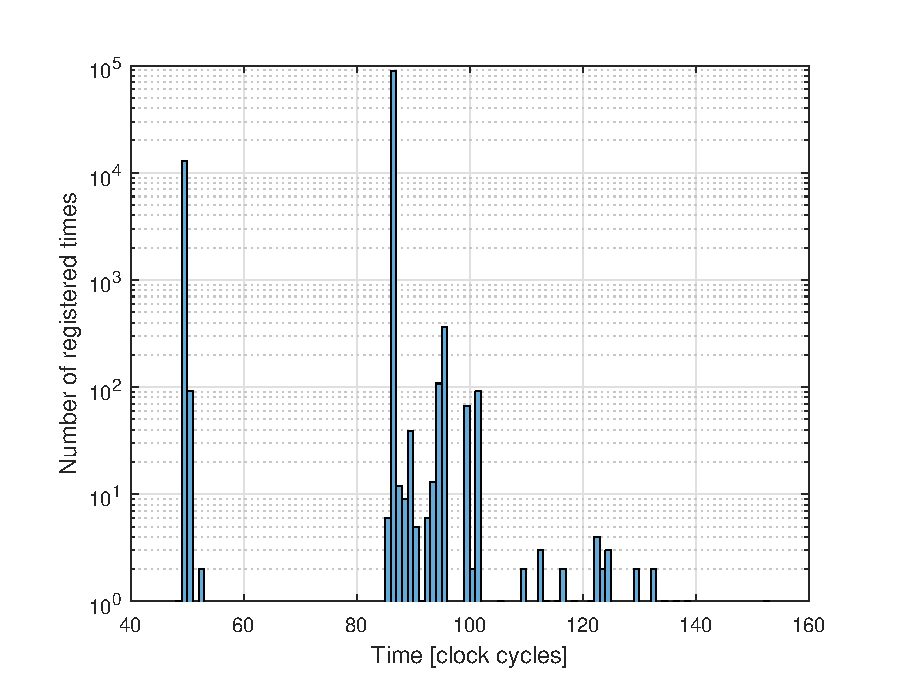
\includegraphics[width=\textwidth]{./img/results_switch_et.eps}
\caption{Visualization of execution times for the OS switch. Note the logarithmic y-axis.}\label{fig:switch_et}
\end{figure}

This results in an overhead of 0.6\% for the entire system. The potential useful CPU utilization is 99.4\%, providing that the GPOS uses all of its allocated CPU time. Using only the RTOS without the hypervisor the CPU utilization would be 0.005\%.\\

Theoretically, if FMP would allow for shorter periods for a task, the maximum overhead for this system would be 24\%.

\section{Hypervisor robustness}
To test the robustness of the hypervisor, a fork bomb was made on the GPOS. A fork bomb is a function that calls itself two times. This quickly depletes the system of its resources, causing it to crash eventually~\cite{forkbomb}. The test resulted in the GPOS crashing and becoming non-responsive while the RTOS managed to maintain all its functionality.\\

%Unregistered exception for a processor core was possible to create by accessing restricted AXI bus address, causing the processor to stop.\\

\chapter{Discussion}
This chapter will discuss the results produced by the thesis.

\section{Robustness}
It is important to know that a hypervisor can never increase robustness of a single OS, only make it more isolated from errors from another OS. Potentially, the hypervisor itself can become the source of an error causing the collective system to fail, see figure~\ref{fig:monitor}.

\begin{figure}[H]
\centering
\begin{subfigure}[b]{0.45\textwidth}
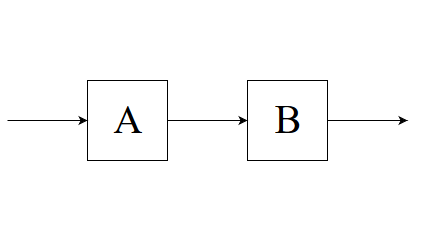
\includegraphics[width=\textwidth]{./img/discussion_nomonitor.png}
\caption{Integrity of A is dependent on integrity of B.}
\end{subfigure}
\begin{subfigure}[b]{0.45\textwidth}
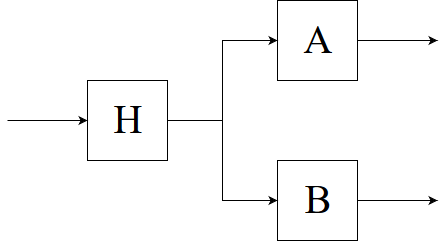
\includegraphics[width=\textwidth]{./img/discussion_monitor.png}
\caption{Integrity of A is isolated from B, but is instead dependent on H.}
\end{subfigure}
\caption{}
\label{fig:monitor}
\end{figure}

Keeping this in mind is important when discussing the robustness of a MCS.

%Adding a new link to a chain can never increase the chains strength, but hopefully the new link is strong enough to not decrease the chains strength. Much like this analogy, the robustness of a system with a hypervisor can not be as good as one without a hypervisor potentially can be. If a system only is dependant on one function to not fail, adding a new function in series can never increase robustness.

\section{Information retrieval}
%Printing to SYSLOG takes time and has an effect on the system that is being monitored.\\
The hardware timer used when measuring execution times requires very little processor time, but still some. This adds an ever so slight error to the execution times. The data was deemed to be of good enough quality anyway.

%\section{Errors}
%Unregistered exception, accessing restricted AXI bus address. Should be avoided by accessing via OS instead of address. All address space should be handled by the OS/monitor, allowing or restricting access to certain address spaces. Probably not correctly setup.

\section{Virtualization resource gain vs resource loss}
%At what point is it not worth it to have a non-critical system application on the same hardware? 
As described earlier, higher frequencies of RTOS tasks leads to more overhead. Disregarding the maximum frequency of 1~kHz for tasks in FMP, the maximum frequency for the functions in the implemented system would be just under 40 kHz, leading to an overhead of 24\% for the hypervisor. This gives the GPOS no time at all for the case when every other task executes for its WCET. However, assuming every task executes for its median execution time, the GPOS can execute for 31\% of the time at 40~kHz. This gives a very good combination of throughput for the entire system and real-time guarantees for the safety-critical tasks at the cost of a maximum overhead of 24\%. This is visualized in figure~\ref{fig:cpu_util}.

\begin{figure}[H]
\centering
\begin{subfigure}[b]{0.49\textwidth}
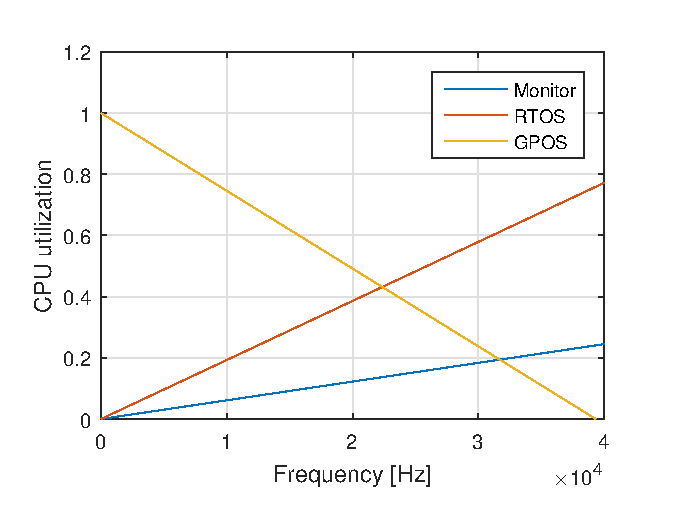
\includegraphics[width=\textwidth]{./img/discussion_util_wcet.eps}
\caption{Worst case execution time}
\end{subfigure}
\begin{subfigure}[b]{0.49\textwidth}
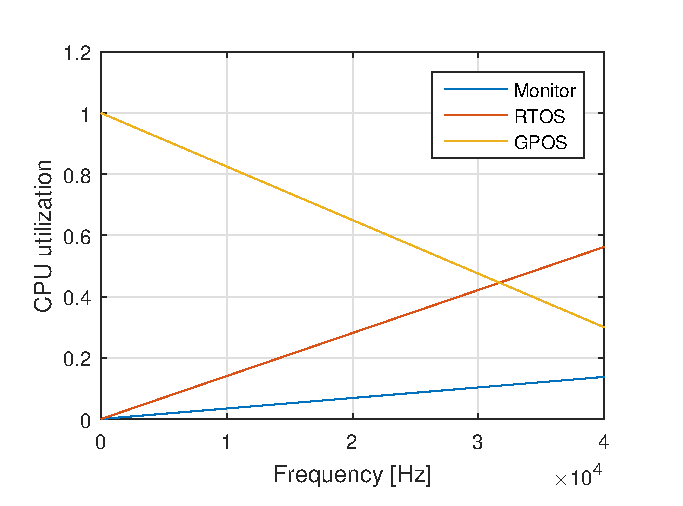
\includegraphics[width=\textwidth]{./img/discussion_util_med.eps}
\caption{Median execution time}
\end{subfigure}
\caption{CPU utilization of monitor, RTOS and GPOS. Note that for the WCET of tasks, 100\% CPU utilization by the monitor and RTOS is reached just before 40 kHz.}
\label{fig:cpu_util}
\end{figure}

%Deterministic system - work towards 100\%, anything under that: reduce clock frequency to reduce power consumption and reach 100\%.\\

%Sporadic system - probably want to be around ~50\% utilization to maintain 100\% schedulability, higher depending on requirements on performance versus requirements on efficiency.

\section{Conclusion}
In the introduction of this thesis, the following research question was presented:

\begin{itemize}
\item Is virtualization an efficient approach when trying to reconcile the conflicting requirements of partitioning for safety assurance and sharing for efficient resource usage when implementing a safety-critical control system?
\end{itemize}

After the implementation, it can be clearly seen that virtualization can be a very efficient and secure approach for reconciling the conflicting requirements of partitioning and sharing. However, finding out if it is efficient in the industry as a whole requires additional research in technical aspects as well as other aspects such as management and financial related ones. These are presented in chapter~\ref{sec:future_work}.

\newpage
\mbox{}

\chapter{Future work}
This chapter will contain thoughts and ideas for future work building on this thesis.
\bibliography{bib}
\appendix
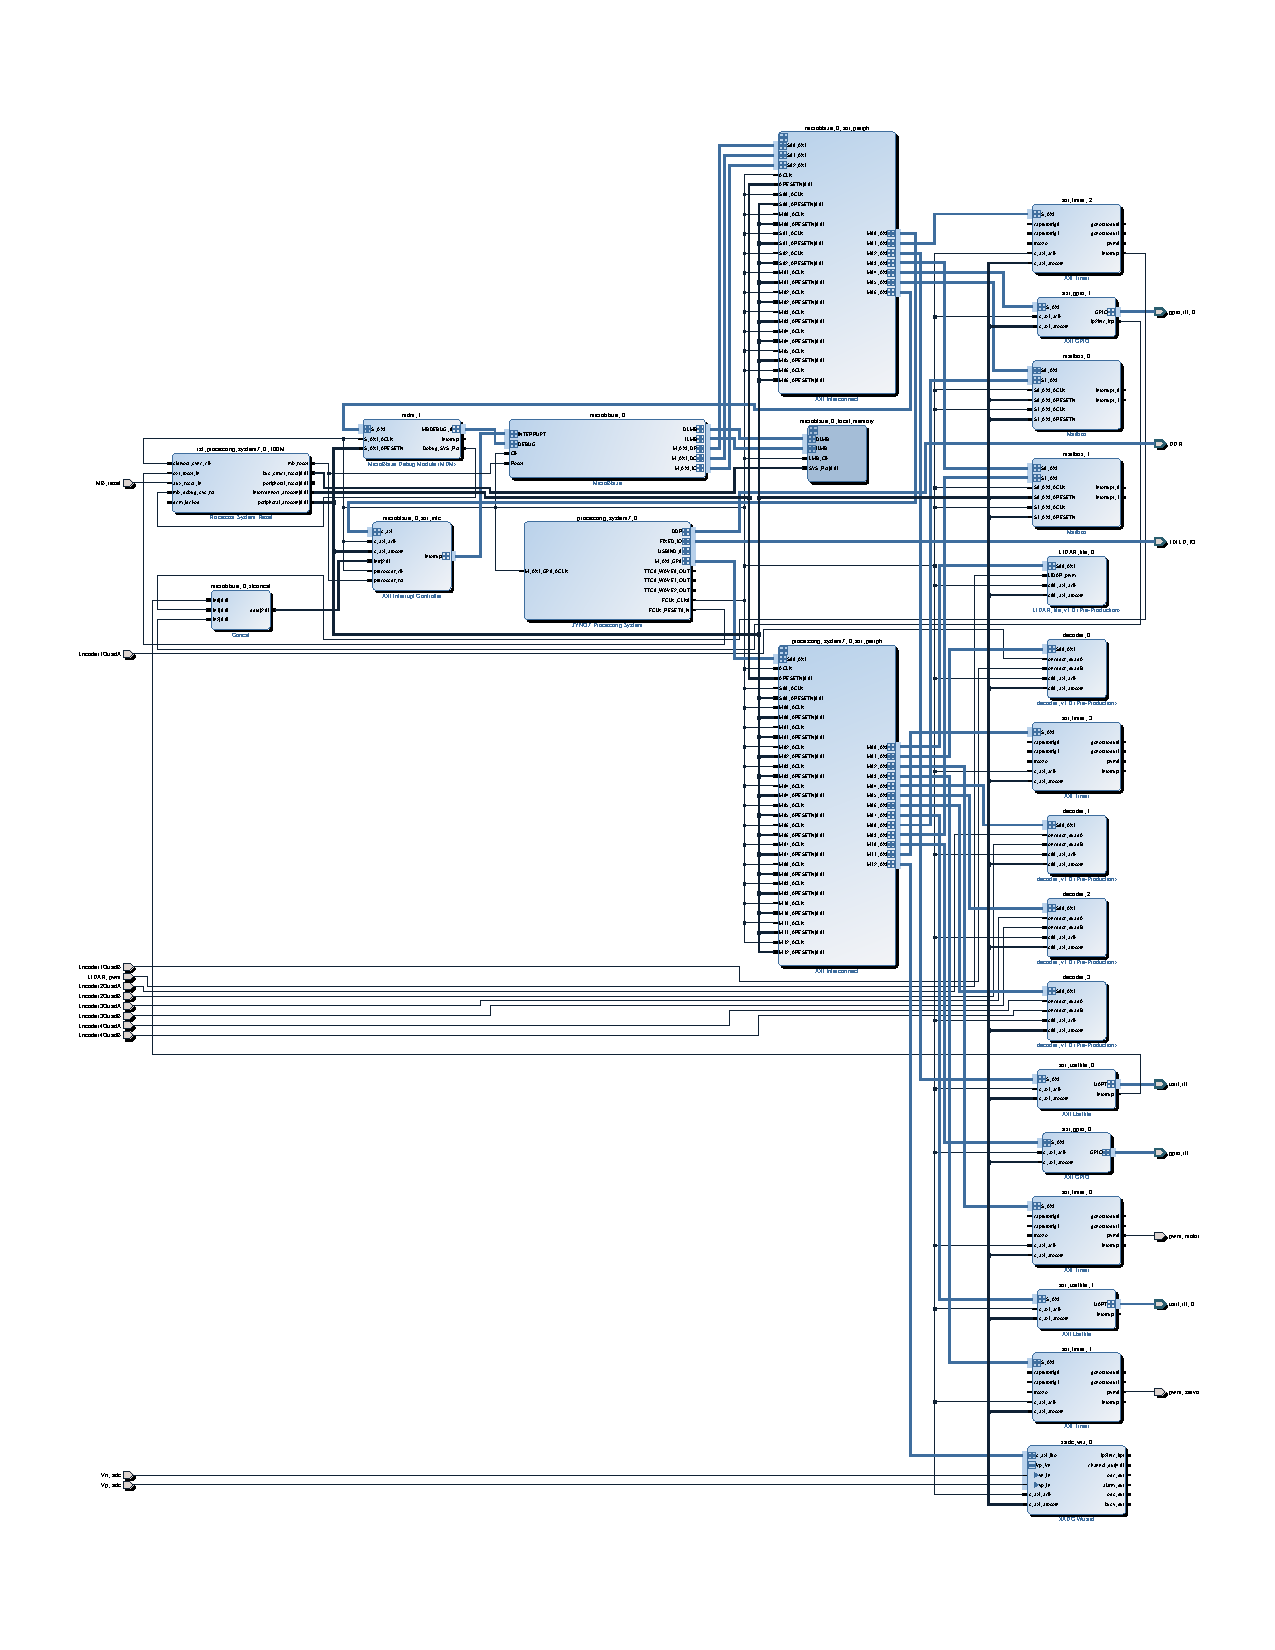
\includepdf[pages=-]{appendices/design_1.pdf}
\label{appendix:A}
\end{document}